\documentclass[aspectratio=169,10pt]{beamer}
\graphicspath{{figures/}} % Setting the graphicspath

% Theme settings
\usetheme{Madrid}
\usecolortheme{default}
\setbeamertemplate{navigation symbols}{}   % removes navigation symbols such as 'next page'
\setbeamertemplate{footline}{}             % remove line with name, date, page nr.
\setbeamercolor*{frametitle}{bg=white}     % remove background from frametitle
\usepackage{caption}
% \captionsetup[figure]{labelformat=empty}% redefines the caption setup of the figures environment in the beamer class.
\setbeamersize{text margin left=20pt,text margin right=10pt}

\usefonttheme[onlymath]{serif} % makes beamer math look like article math


%======================= import packages =======================
\usepackage{graphicx}     % More options for \includegraphics
\usepackage{appendixnumberbeamer} % separate appendix numbering
\usepackage{url}
\usepackage{hyperref}
\usepackage{booktabs}
\usepackage{xcolor}

\definecolor{amethyst}{rgb}{0.6, 0.4, 0.8} % for the hopscotch chi2 table

%======================= page numbering =======================
\addtobeamertemplate{navigation symbols}{}{ \usebeamerfont{footline}
  \insertframenumber / \inserttotalframenumber \hspace*{2mm} \\ \vspace*{1mm}
}


\newcommand{\chitwo}{$\chi^2$}

%=================================== colors ===================================
\definecolor{RoyBlue}{RGB}{22, 46, 69}
\definecolor{RoyGrey}{RGB}{64, 88, 128}

\newcommand{\hlme}[1]{{\color{red}\bf #1}} % highlihgt me

\setbeamercolor{structure}{fg=RoyBlue} % itemize, enumerate, etc
\setbeamercolor{frametitle}{fg=RoyGrey}
\setbeamercolor{section in head/foot}{bg=RoyBlue}


%======================= add progress dots to headline =======================
\setbeamertemplate{headline}{%
    \begin{beamercolorbox}[ht=4mm,dp=4mm]{section in head/foot}
        \insertnavigation{\paperwidth}
    \end{beamercolorbox}%
}%
\makeatother


%======================= add section title page =======================
\AtBeginSection[]{
  \begin{frame}
  \vfill
  \centering
    \usebeamerfont{title}\insertsectionhead\par%
  \vfill
  \end{frame}
}


%================================== TITLEPAGE ==================================
\title{Hopscotch: a quick recap}
\date{NNPDF meeting, 30 August 2022, Gargnano}
\author{Roy Stegeman}
\institute{University of Milan and INFN Milan}
\titlegraphic{\vspace*{6mm}
    
\includegraphics[height=0.8cm]{logos/LOGO-ERC.jpg} \hspace{10mm}
	
\includegraphics[height=0.8cm]{logos/n3pdflogo_noback.png} \hspace{10mm}
	
\includegraphics[height=0.6cm]{logos/nnpdf_logo_official.pdf} \hspace{10mm}
	\includegraphics[height=0.8cm]{logos/Logo_Università_degli_Studi_di_Milano(not_mandatory).png}
	
\includegraphics[height=0.8cm]{logos/INFN_logo.png}
    \vspace*{5mm} \\
	\centering{
	\fontsize{7.0pt}{0.0pt}\selectfont This project has received funding from the European Union’s Horizon 2020 \\
    \vspace*{-1mm}
	research and innovation programme under grant agreement No 740006.
	}
}




%================================== SLIDES ==================================

\begin{document}
{
\setbeamertemplate{headline}{} % remove headline from titlepage
\begin{frame}
  \titlepage
\end{frame}
}



\section{The hopscotch scan}

\begin{frame}[t]{The hopscotch scan}{From \url{https://arxiv.org/pdf/2205.10444.pdf}}
  Hopscotch replicas are generated by sampling along Hessian eigenvector directions that result in large changes to $\sigma_H$ and $\sigma_Z$
  \begin{figure}
    \centering
    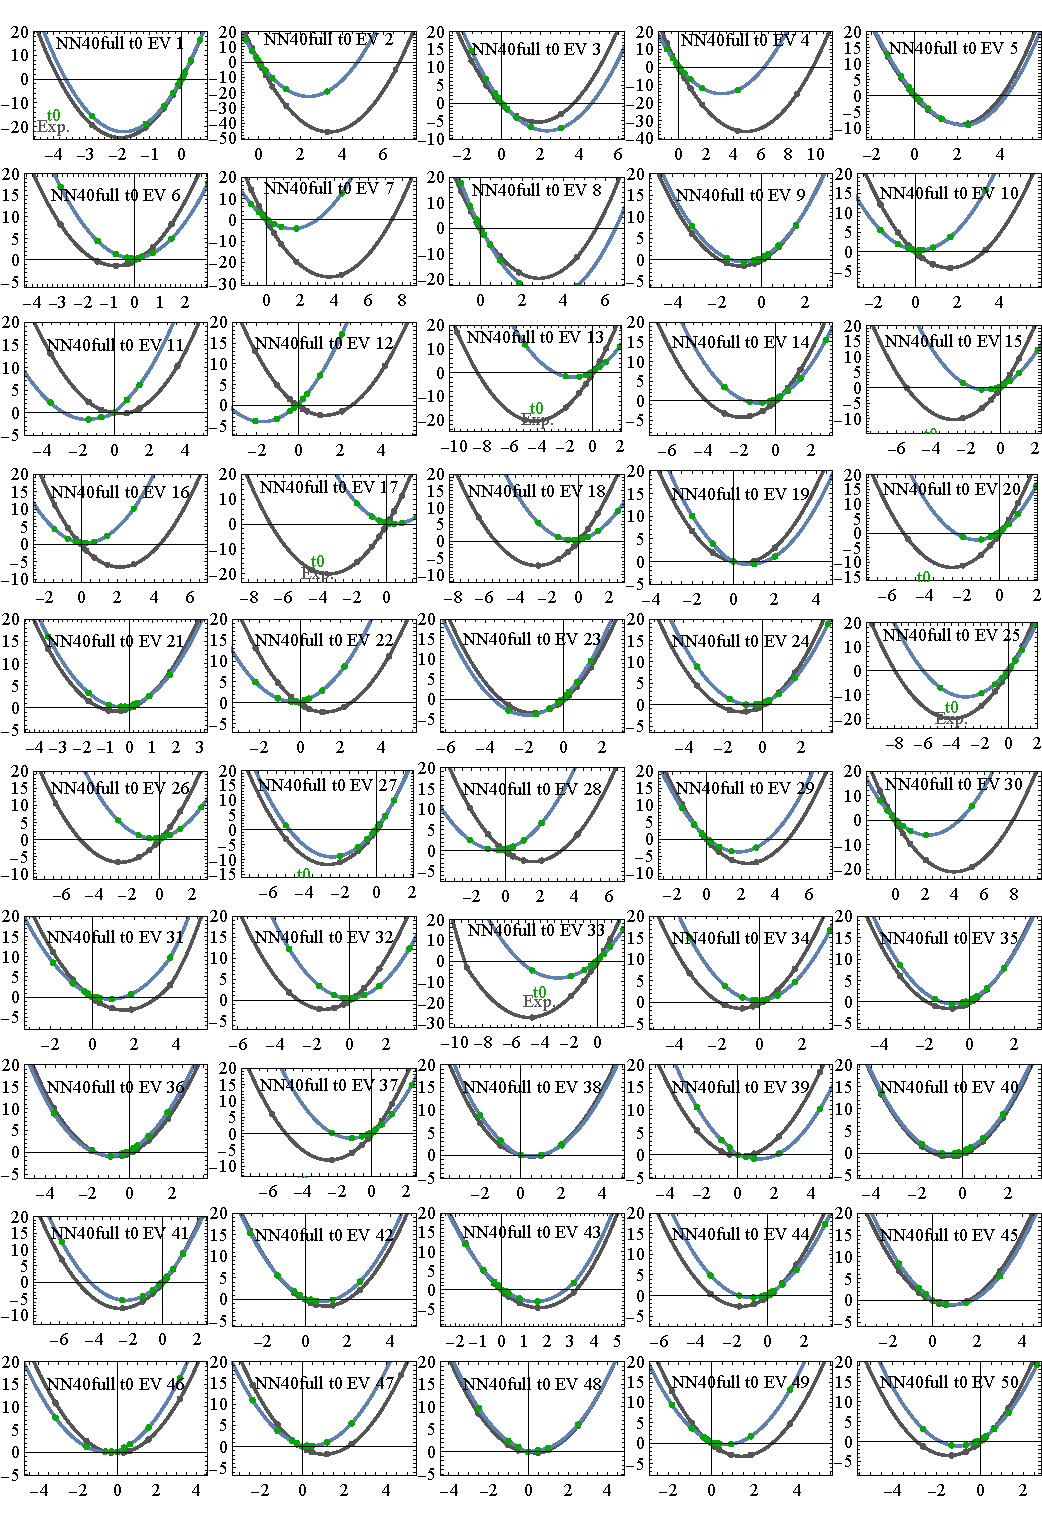
\includegraphics[width=.2\textwidth]{220510_t0_vs_exp_parabolas.pdf}
    \hspace*{1em}
    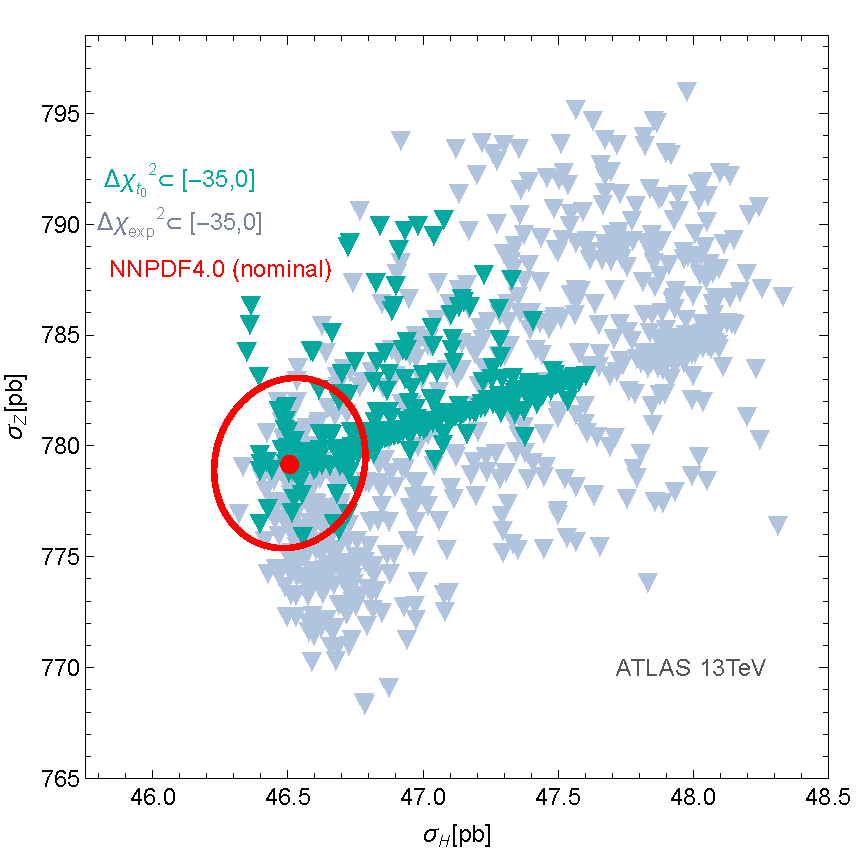
\includegraphics[width=.3\textwidth]{220512_scatter_HZ_exp_t0.pdf}
    \caption*{The paper contains two figures that consider the $t_0$ prescription, Fig. 6 (left) and Fig. 7 (right)}
  \end{figure}
\end{frame}

\begin{frame}[t]{Where are the negative $\Delta\chi^2_{t_0}$ solutions?}
  The ``outside'' replicas are defined by drawing a rectangular box around the NNPDF4.0 predictions.\\
  \vspace*{0.5em}
  All outside replicas are defined by larger $\sigma_H$
  \begin{columns}
    \begin{column}{0.48\textwidth}
      \vspace*{-1mm}
      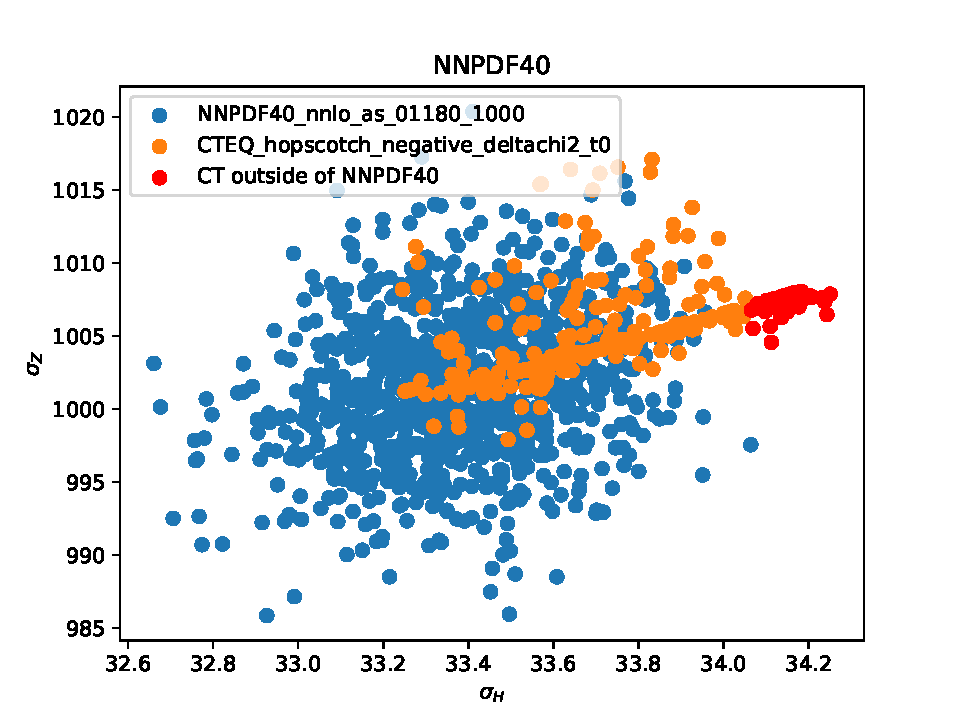
\includegraphics[width=.9\textwidth]{NNPDF40.pdf}
    \end{column}
    \hspace*{0.01\textwidth}
    \begin{column}{0.48\textwidth}
      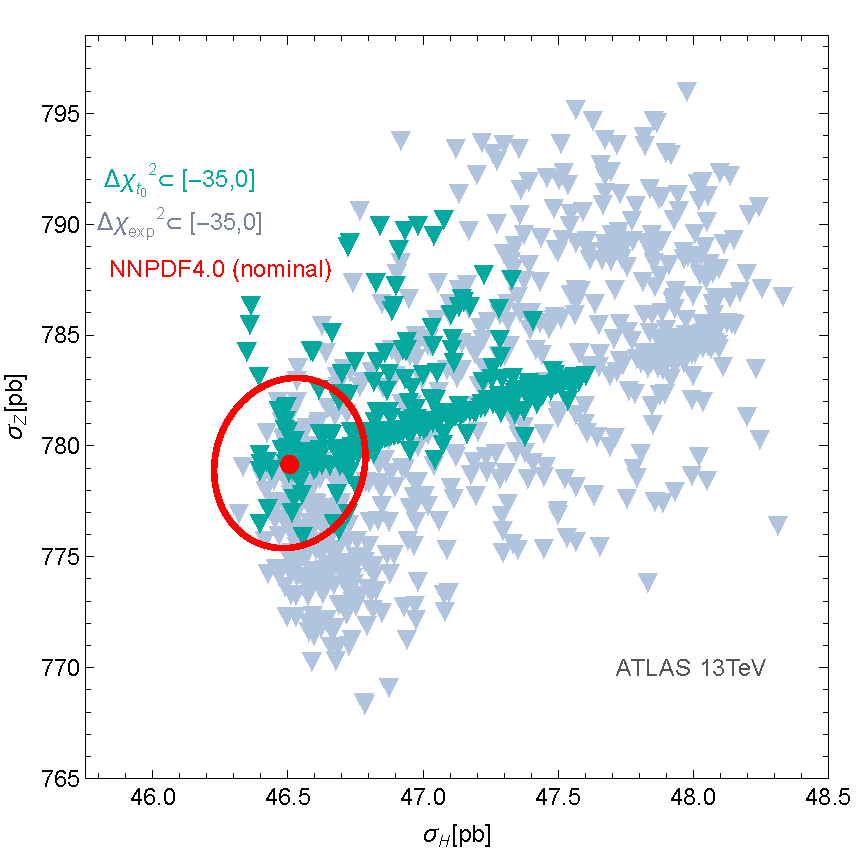
\includegraphics[width=.7\textwidth]{220512_scatter_HZ_exp_t0.pdf}
    \end{column}
  \end{columns}
\end{frame}

\begin{frame}[t]{The LO differential cross-section}
  Most of the discrepancy is in the low rapidity $y$ region\\
  \vspace*{0.5em}
  discrepancy is there at LO, suggesting a shift of the $gg$ luminosity
  \begin{center}
    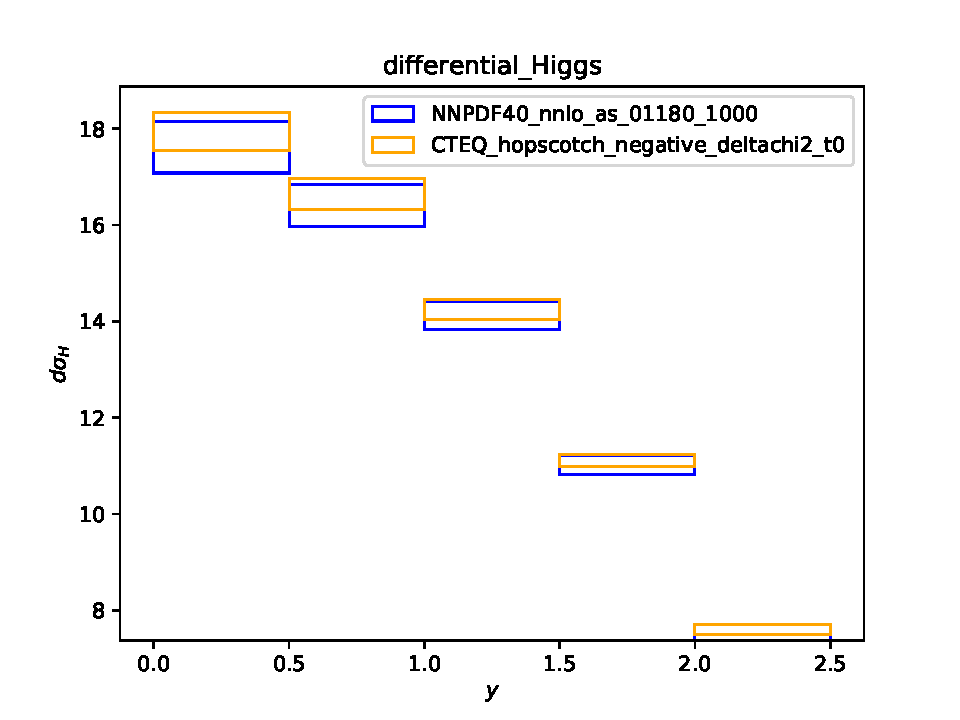
\includegraphics[width=.48\textwidth]{differential_Higgs.pdf}
    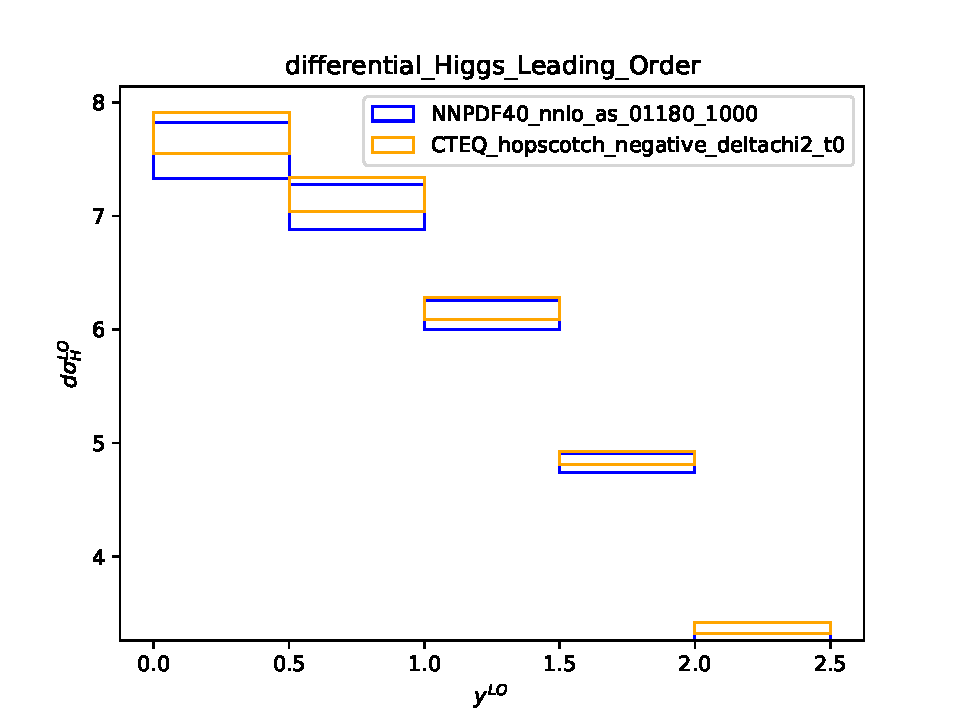
\includegraphics[width=.48\textwidth]{differential_Higgs_Leading_Order.pdf}
  \end{center}
\end{frame}

\begin{frame}[t]{What PDF feature dominates the discrepancy?}
  Around the Higgs mass the luminosities of the hopscotch outliers are outside the region that has been sampled by NNPDF4.0\\
  \begin{center}
    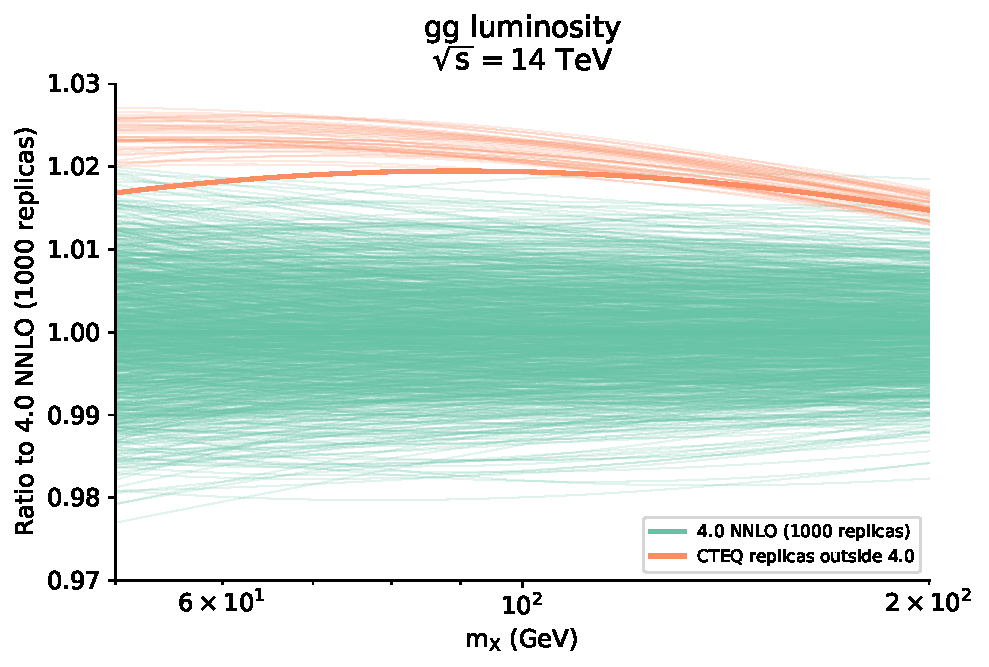
\includegraphics[width=.48\textwidth]{plot_lumi1d_replicas.pdf}
  \end{center}
\end{frame}


\begin{frame}[t]{What PDF feature dominates the discrepancy?}
  There is a clear kink in the hopscotch gluon PDFs, does this correspond to a deterioration of the PDFs?
  \begin{columns}
    \begin{column}{.38\textwidth}
      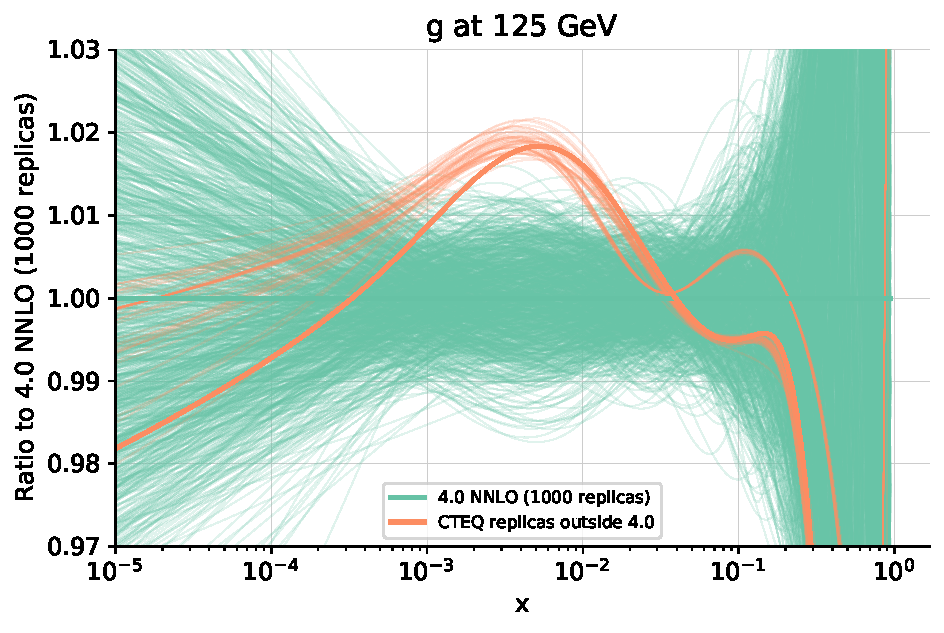
\includegraphics[width=4cm]{plot_pdfreplicas_g.pdf}\\
      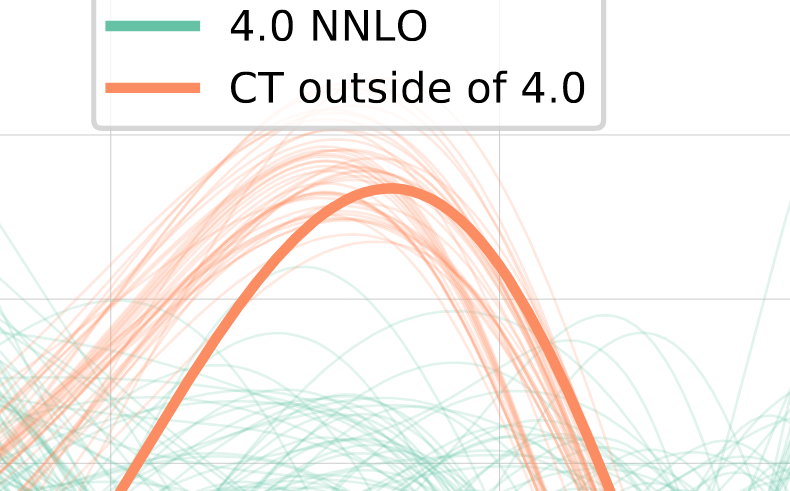
\includegraphics[width=4cm]{zoomin.png}
    \end{column}
    \begin{column}{.6\textwidth}
      \begin{tabular}{lr|r|r|r}
        \toprule
        group &  n &  NNPDF 40 $\chi^{2}$ &  CTEQ $\chi^{2}$ \\
        \midrule
        DIS NC &        2100 &    1.218623 &  1.210005 \\
        DIS CC &         989 &    0.893750 &  0.881195 \\
        \color{blue} DY &         893 &   \color{blue} 1.261028 & \color{blue} 1.226119 \\
        \color{red} TOP &          66 &   \color{red}  1.210918 & \color{red}  1.312839 \\
        \color{amethyst} JETS &         356 &     \color{amethyst} 0.943735 &  \color{amethyst} 0.879847 \\
        DIJET &         144 &    2.007296 &  1.991372 \\
        PHOTON &          53 &    0.763523 &  0.787850 \\
        SINGLETOP &          17 &    0.363610 &  0.352023 \\
        \bottomrule
      \end{tabular}
    \end{column}
  \end{columns}
\end{frame}



\section{Study so far}

\begin{frame}[t]{`everthing' seems to find the CT solutions}
  \vspace*{-1.5em}
  \begin{columns}
    \begin{column}{.28\textwidth}
      Only the full NNPDF4.0 dataset together seems unable to find the CT solutions
    \end{column}
    \begin{column}{.7\textwidth}
      \centering
      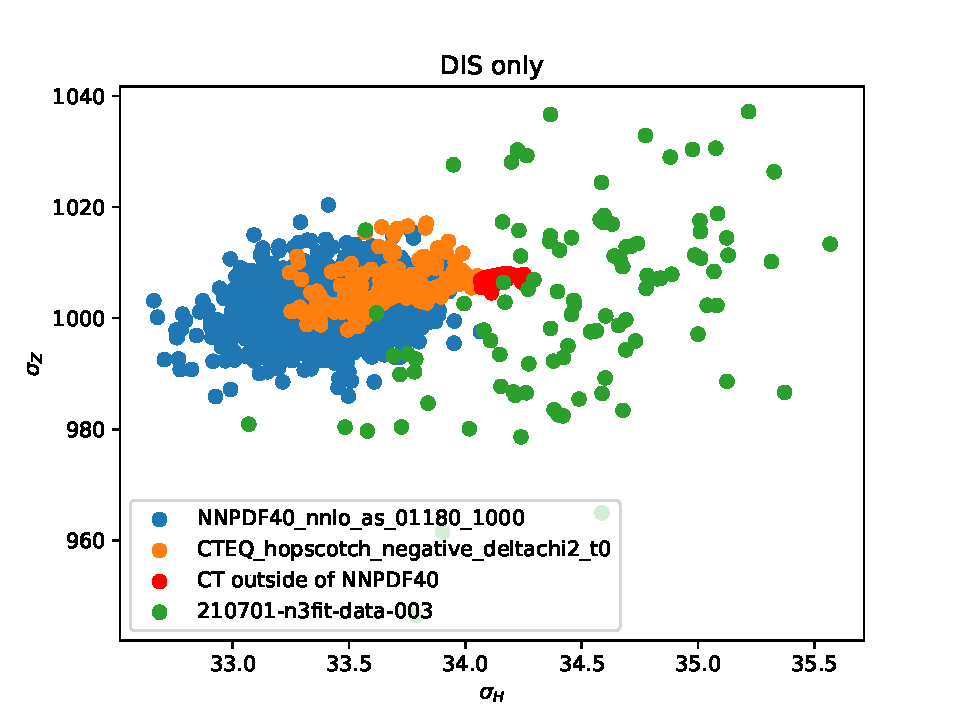
\includegraphics[height=.45\textheight]{DIS_only.pdf}
      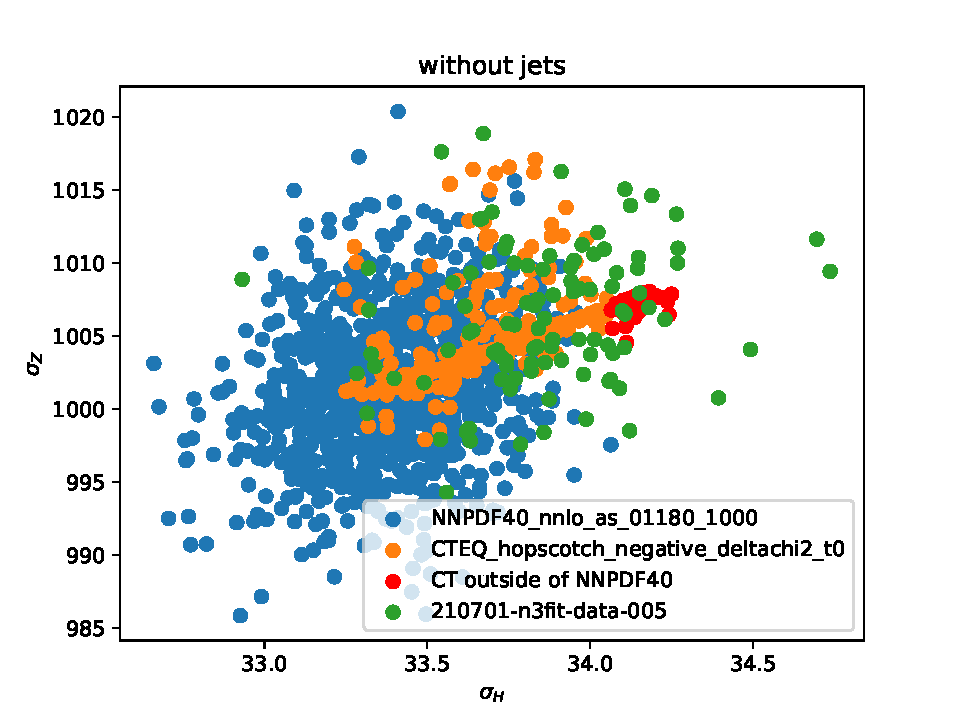
\includegraphics[height=.45\textheight]{without_jets.pdf}\\
      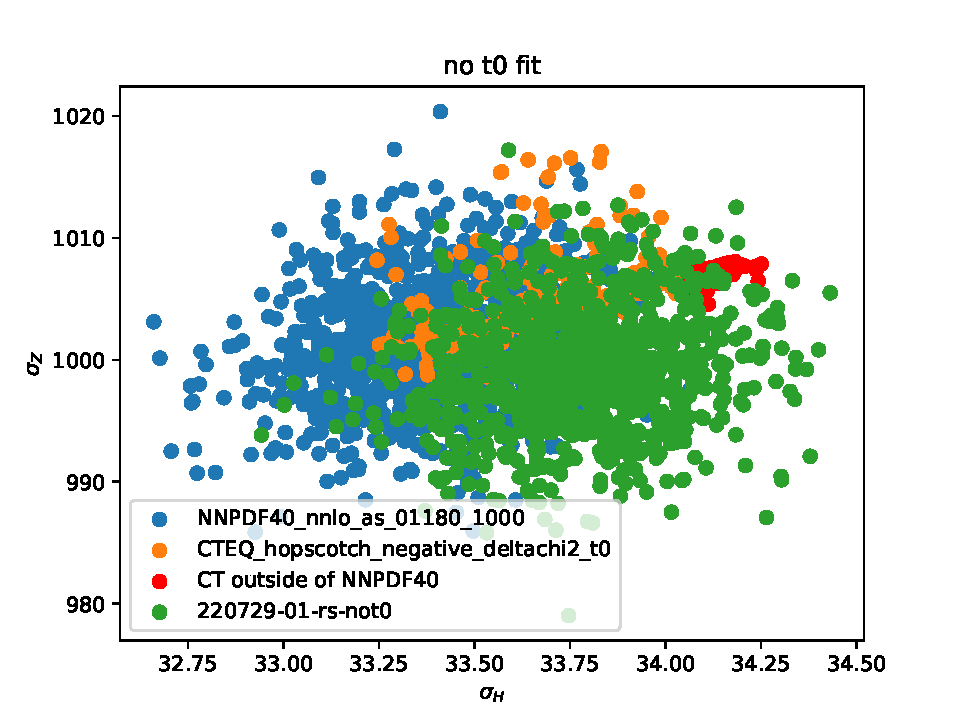
\includegraphics[height=.45\textheight]{no_t0_fit.pdf}
      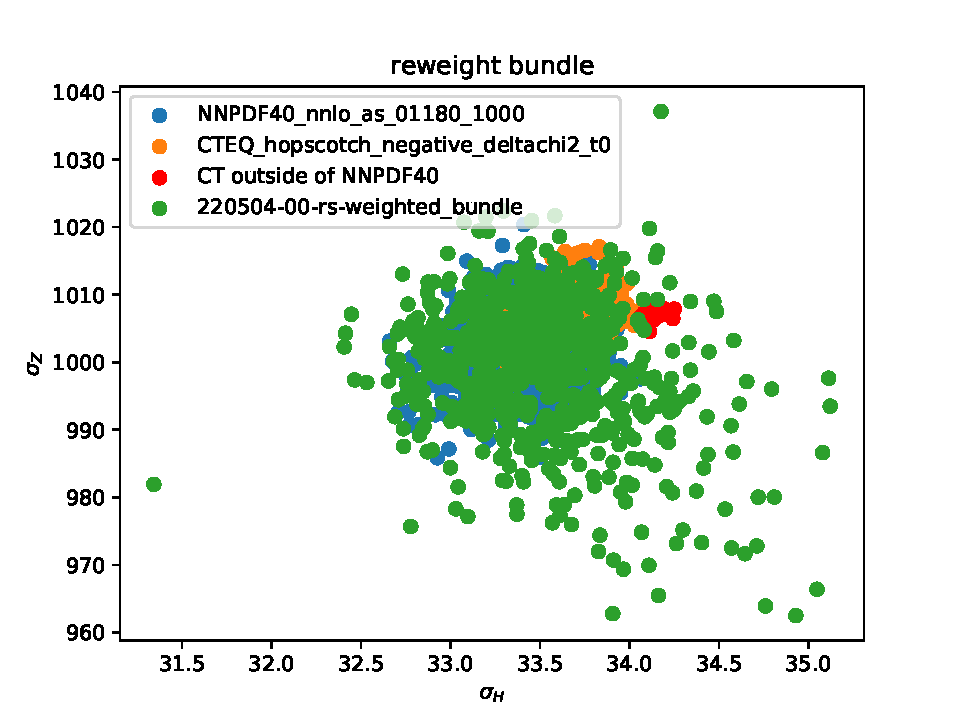
\includegraphics[height=.45\textheight]{reweight_bundle.pdf}
    \end{column}
  \end{columns}
\end{frame}

\begin{frame}[t]{training/validation, overfitting}
  Remember that the \chitwo improved for some processes while it deteriorated for others, this may suggest early-stopping prevents us from finding these solutions.\\\vspace*{.5em}
  However, even without a training/validation split, the CT solutions are not found:
  \begin{figure}
    \centering
    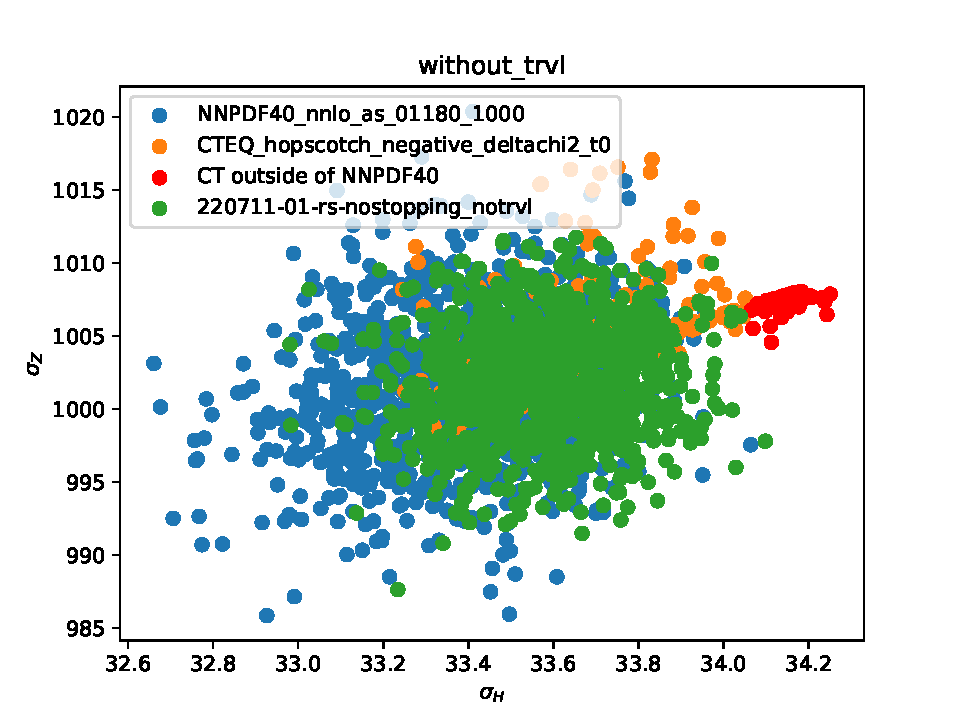
\includegraphics[height=.55\textheight]{without_trvl.pdf}
  \end{figure}
\end{frame}

\begin{frame}[t]{training/validation, overfitting}
  Looking at the \chitwo distribution, the direction of the CT replicas does seem to correspond to lower values
  \begin{figure}
    \centering
    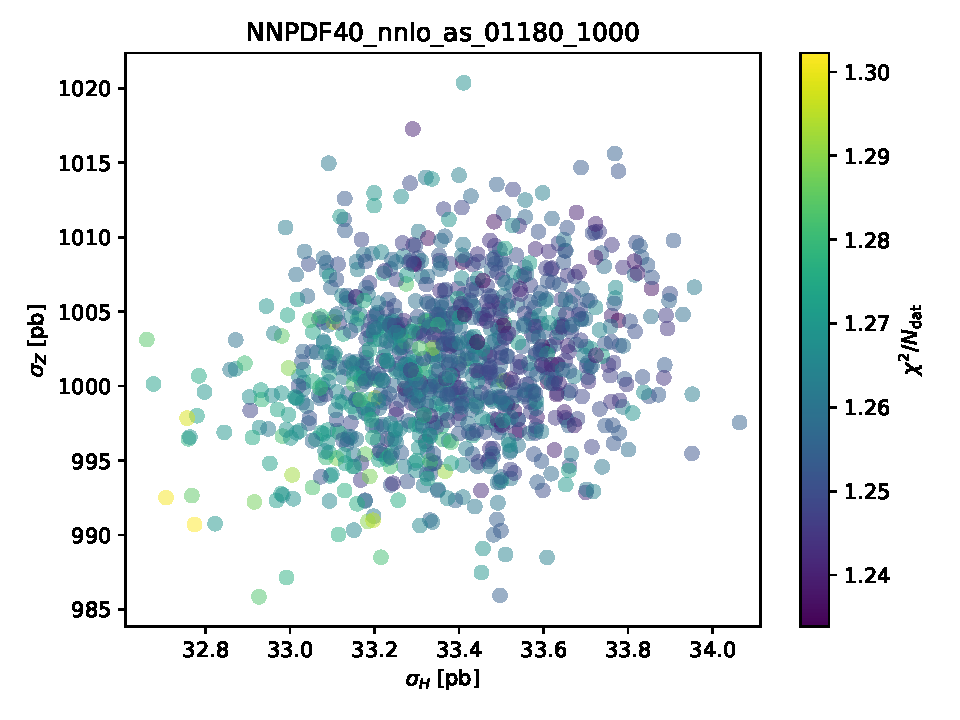
\includegraphics[height=.55\textheight]{nnpdf40_chi2_scatter.pdf}
    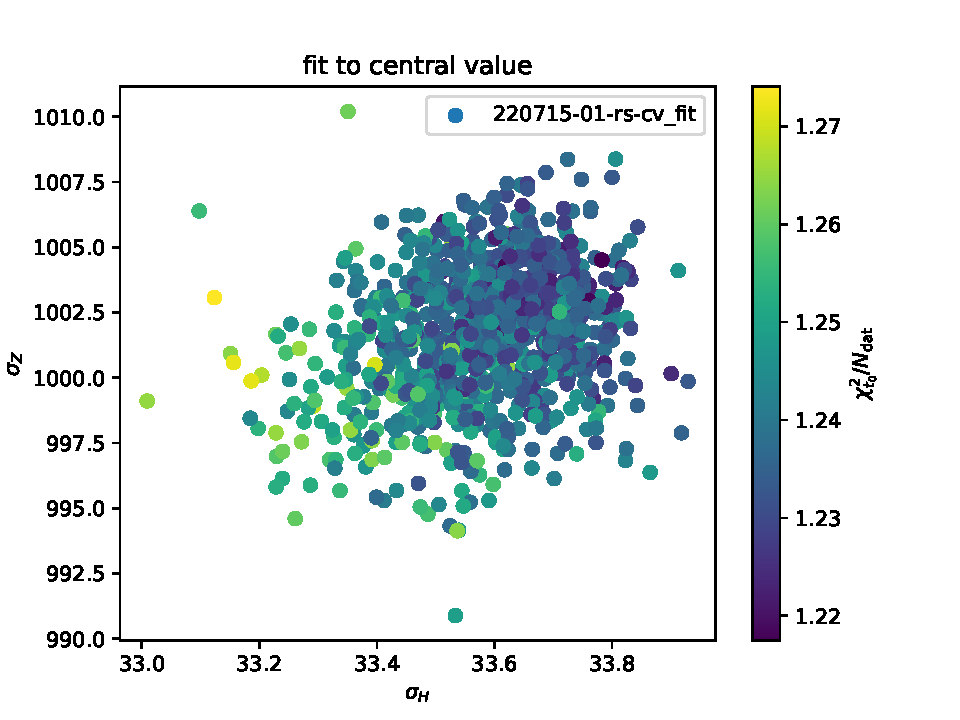
\includegraphics[height=.55\textheight]{chi2_fit_to_central_value.pdf}
  \end{figure}
\end{frame}

\begin{frame}[t]{training/validation, overfitting}
  Though training and validation losses seem uncorrelated with the value their position in the $\sigma_H,\sigma_Z$ plane
  \begin{figure}
    \centering
    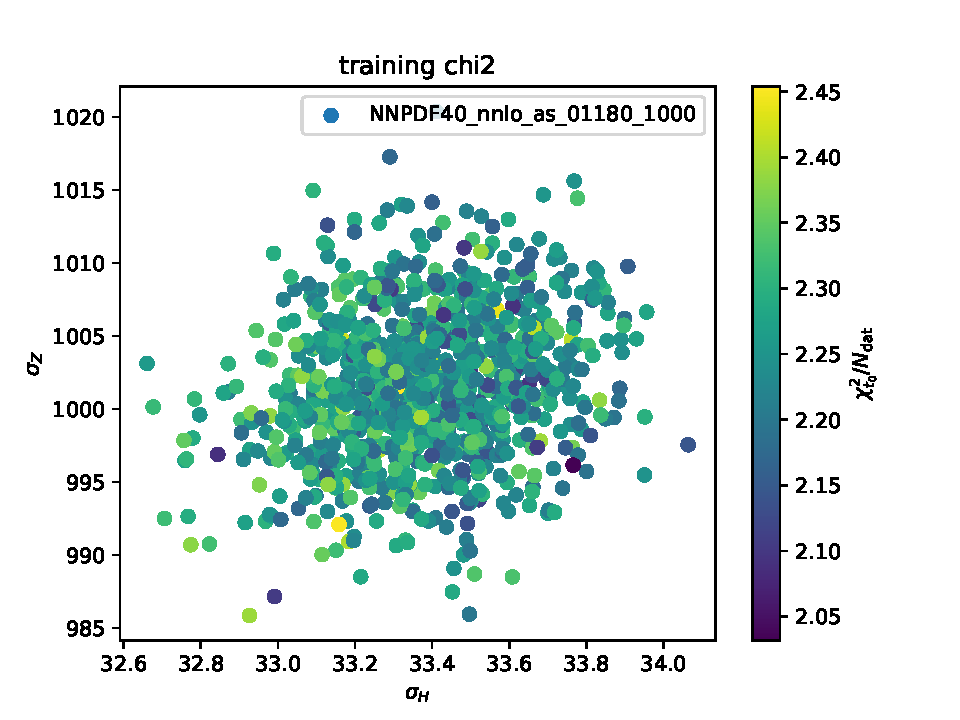
\includegraphics[height=.55\textheight]{chi2_training_chi2.pdf}
    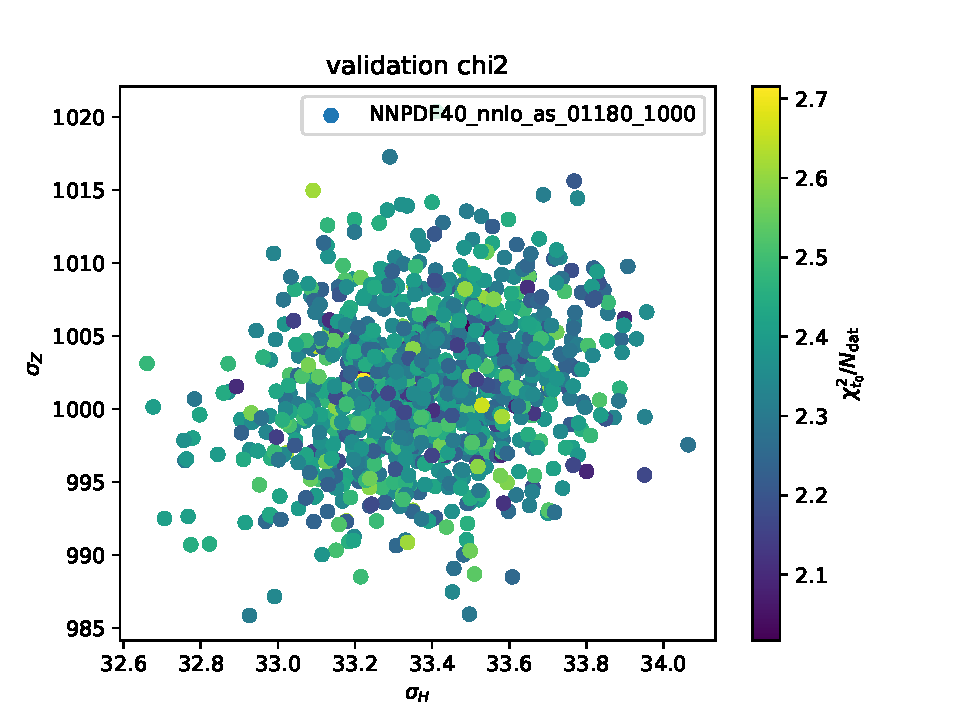
\includegraphics[height=.55\textheight]{chi2_validation_chi2.pdf}
  \end{figure}
\end{frame}


\begin{frame}[t]{The impact of phyicsl constraints}
  While dataset variations seem to generate solutions in the CT region, this does not seem the case when the physical constraints are relaxed.
  \begin{figure}
    \centering
    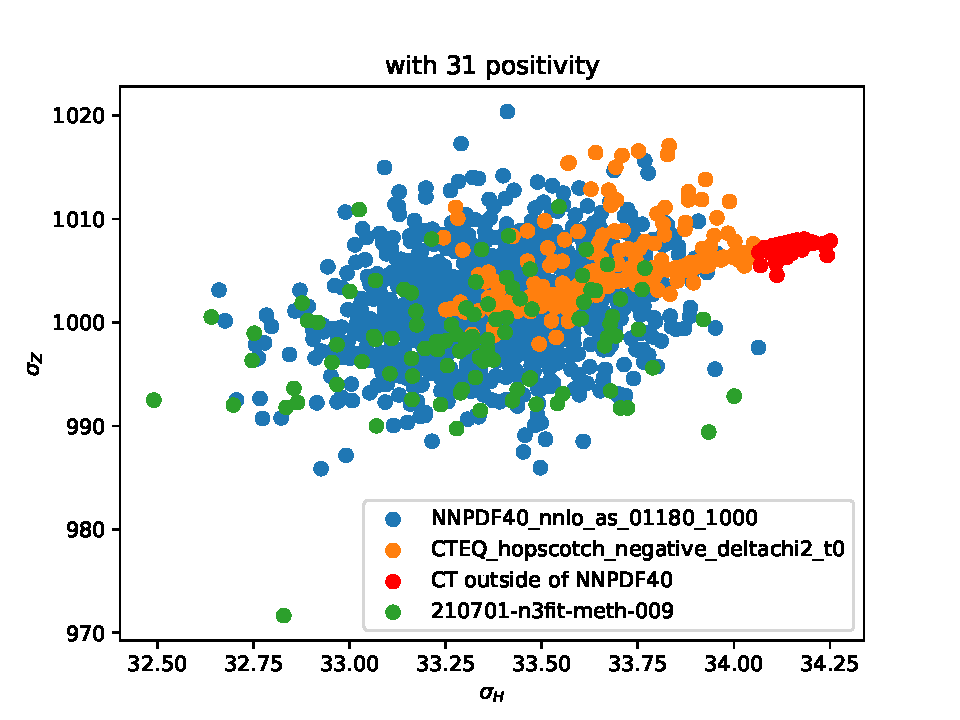
\includegraphics[height=.55\textheight]{with_31_positivity.pdf}
    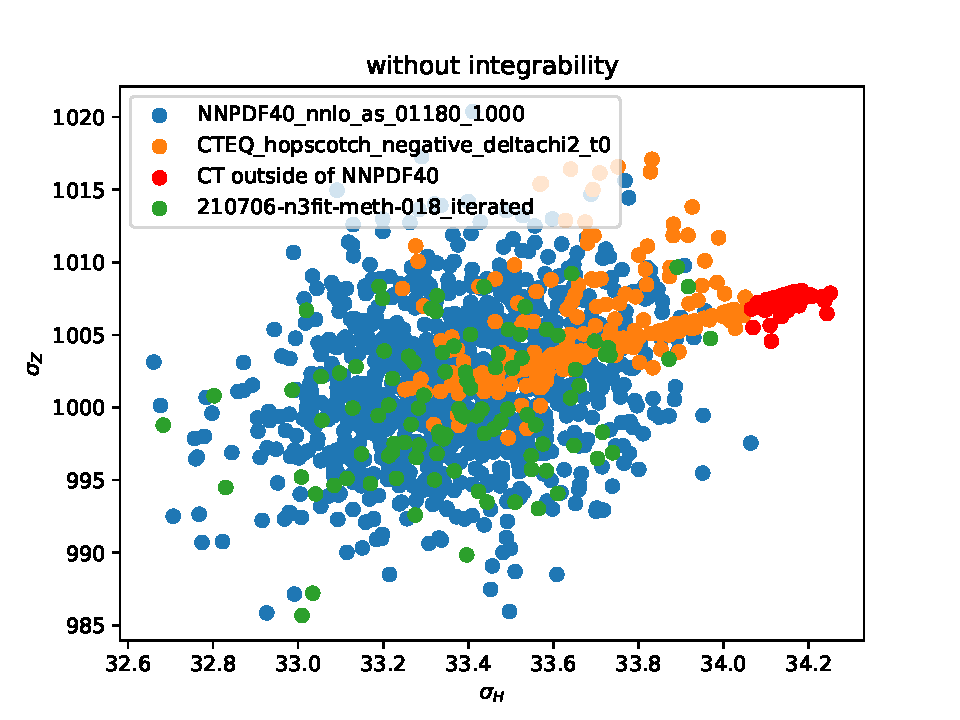
\includegraphics[height=.55\textheight]{without_integrability.pdf}
  \end{figure}
\end{frame}

\begin{frame}[t]{Methodology variations - training fraction}
  If we change the training fraction to 0.50, the training loss increases while the validation loss decreases\\\vspace*{.5em}
  There is no reason to think a fraction of 0.75 is better, and 0.50 is more conservative\\\vspace*{.5em}
  The lack of PDFs in the CT region (as result of a low likelihood?) may in part be understood as a result of the cross-validation regularization
  \begin{center}
    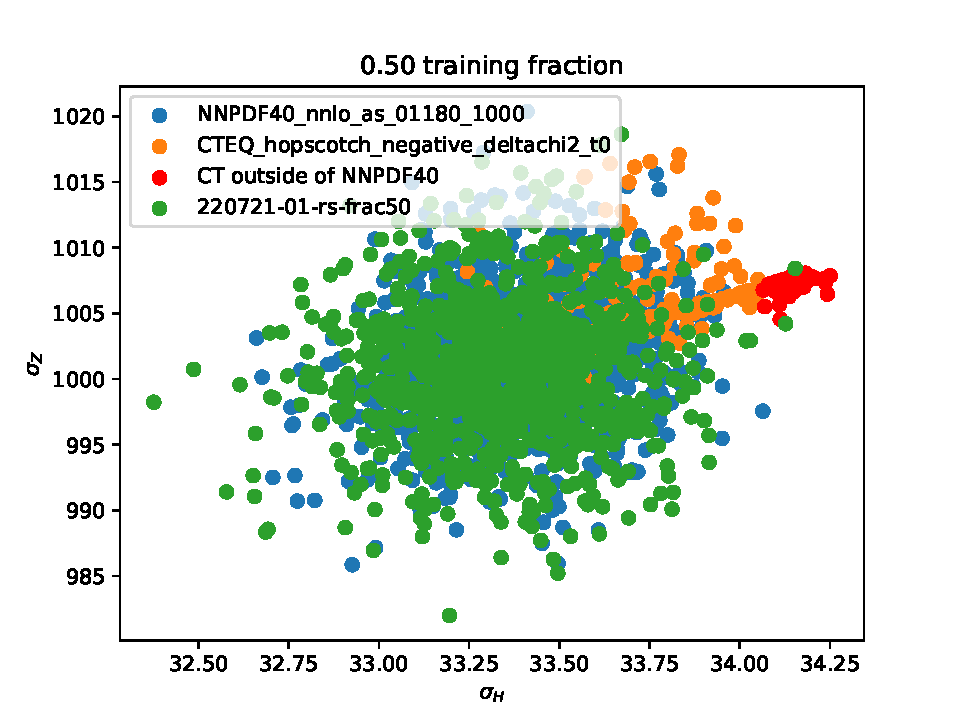
\includegraphics[height=.5\textheight]{0.50_training_fraction.pdf}
    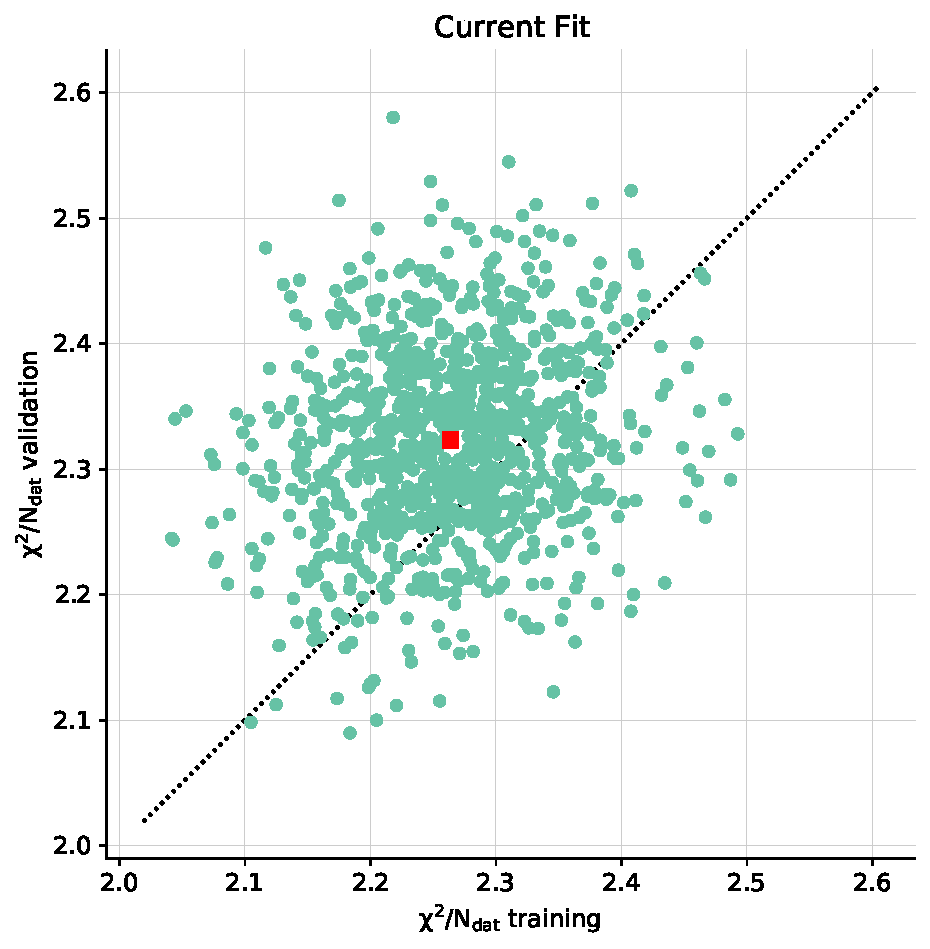
\includegraphics[height=.5\textheight]{frac50_training_validation.pdf}
    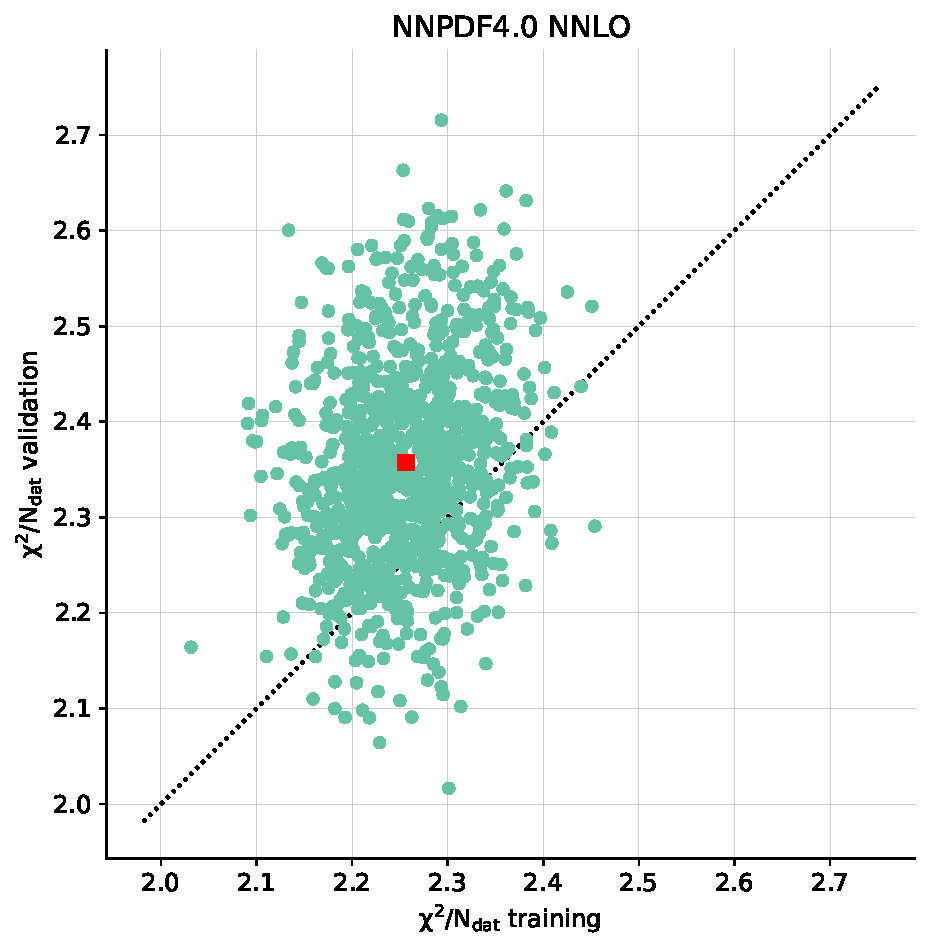
\includegraphics[height=.5\textheight]{NNPDF40NNLO_plot_training_validation.pdf}
  \end{center}
\end{frame}


\begin{frame}[t]{Referee report-like plots, \chitwo per replica}
  \vspace*{-0.1cm}
  No surprises here: if the sample is large enough, we do find replicas with a \chitwo smaller than replica0\\
  \begin{columns}
    \begin{column}{0.5\textwidth}
      \begin{figure}
        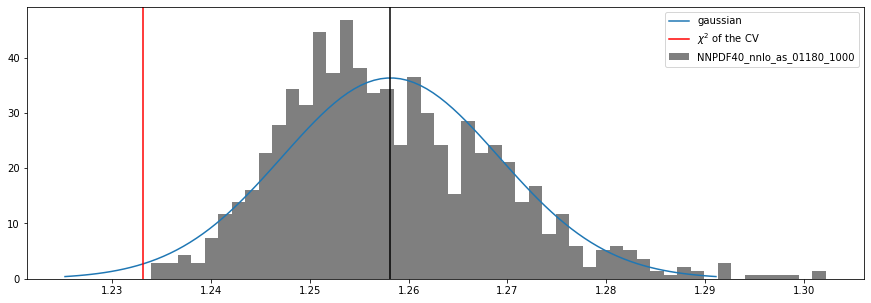
\includegraphics[height=.3\textheight]{chi2_replicas_nnpdf40_1000.png}
        \caption*{\footnotesize NNPDF4.0 (1000 replicas)}
      \end{figure}
      \vspace*{-0.8cm}
      \begin{figure}
        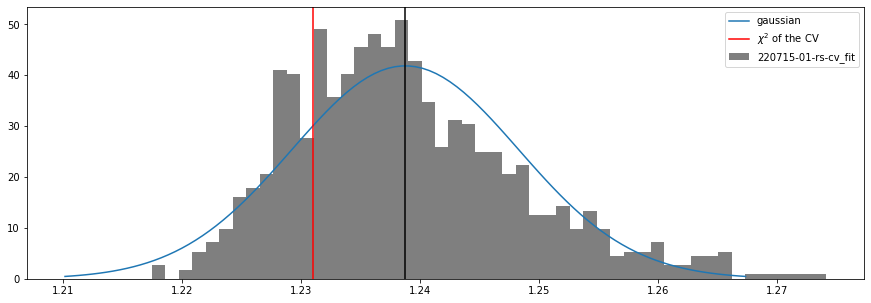
\includegraphics[height=.3\textheight]{chi2_replicas_level1_fit.png}
        \caption*{\footnotesize  fit to experimental central values}
      \end{figure}
    \end{column}
    \begin{column}{0.5\textwidth}
      \begin{figure}
        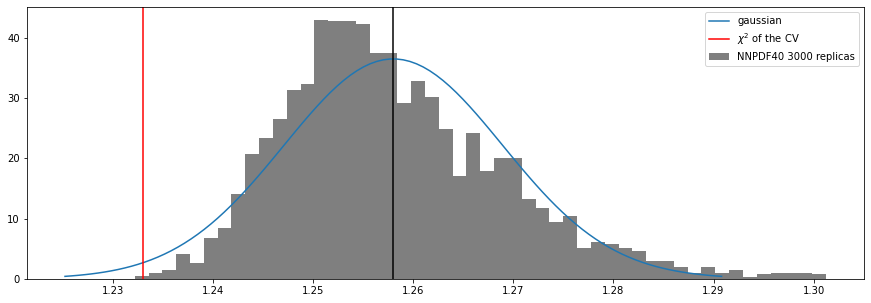
\includegraphics[height=.3\textheight]{chi2_replicas_nnpdf40_3000.png}
        \caption*{\footnotesize  NNPDF4.0 (3000 replicas)}
      \end{figure}
      \vspace*{-0.8cm}
      \begin{figure}
        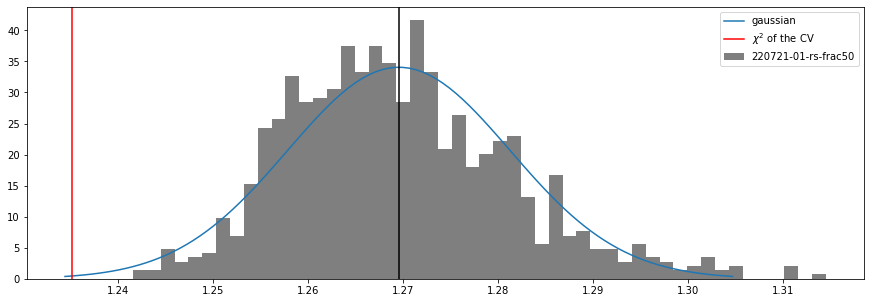
\includegraphics[height=.3\textheight]{chi2_replicas_0.5trvl.png}
        \caption*{\footnotesize  0.50 training fraction}
      \end{figure}
    \end{column}
  \end{columns}
\end{frame}


\section{How to proceed}

\begin{frame}[t]{Understanding what points we need to address}
  There are some critical problems in the understanding of the NNPDF methodology within the wider community as well as other criticisms. Namely, it (by some) believed that:
  \begin{itemize}
    \item $\chi^2$ is a measure of the likelihood
    \begin{itemize}
      \item so \chitwo must be minimum at the best fit
      \item and good \chitwo can't be far away
    \end{itemize}
    \item There must be a reproducible best solution
    \begin{itemize}
      \item There is no unique best solution (even for level-0 data)
    \end{itemize}
    \item NN has unclear assumptions as opposed to a fixed functional form
    \begin{itemize}
      \item Maybe the NN disfavors wiggles where there should be wiggles. The Hessian method avoids this through tolerance
    \end{itemize}
    \item Perhaps more?
  \end{itemize}
  Some of the skepticism seems to have been ignited by the basis independence check in the NNPDF4.0 paper
\end{frame}

\begin{frame}[t]{Organizing the rebuttal}
  So far we have tried to address these criticisms in talks and conversations, but perhaps we should address it in a public document\\
  \vspace*{0.5em}
  Do we understand what arguments we would need to put in the rebuttal?\\
  \vspace*{0.5em}
  What results/checks will we need to do?\\
  \vspace*{2em}

  \textbf{Publishing}\\
  We don't want to be limited to a small number of pages (so no proceedings)\\
  {\footnotesize\qquad P.S. deadline for ICHEP proceedings is 31 October}\\
  \vspace*{0.5em}
  Paper, arxiv preprint, note on website, \ldots. are all options\\
\end{frame}



\begin{frame}{Determination of the photon PDF}
  \begin{columns}[T]
    \begin{column}{0.59\textwidth}
      Initially the photon PDF has been determined in different ways:
      \begin{itemize}
        \item physical model: sensitive to underlying model
        \item fitting: data does not provide strong constraints
      \end{itemize}

      \vspace*{0.5em}
      However with the LUXqed approach it can be computed perturbatively \\
      based on the observation that the heavy-lepton production cross-section can be written in two ways:
      \begin{itemize}
        \item in terms of structure functions $F_2$, $F_L$
        \item in terms of PDFs (including the photon)
      \end{itemize}

      \vspace*{0.5em}
      luxQED result {\color{gray}\small[Manohar, Nason, Salam, Zanderighi: 1607.04266, 1708.01256]}:
      \vspace*{-0.8em}
      \begin{equation*}
        \begin{split}
          & x \gamma(x, \mu^2)
          =
          \frac{2}{\alpha (\mu^2)} \int\limits_x^1 \frac{dz}{z}
          \Biggl\{ \int_{m_p^2x^2 \over 1-z}^{\mu^2 \over 1-z} \frac{dQ^2}{Q^2}
          \alpha^2(Q^2) \Biggl[ -z^2 F_L(x/z, Q^2) \\
          & + \left( z P_{\gamma q}(z) + \frac{2 x^2 m_p^2}{Q^2} \right)
          F_2(x/z, Q^2)\Biggr] - \alpha^2(\mu^2) z^2 F_2(x/z, \mu^2)\Biggr\}
        \end{split}
      \end{equation*}
    \end{column}

    \begin{column}{0.39\textwidth}
      \vspace*{-2.5em}
      \begin{figure}
        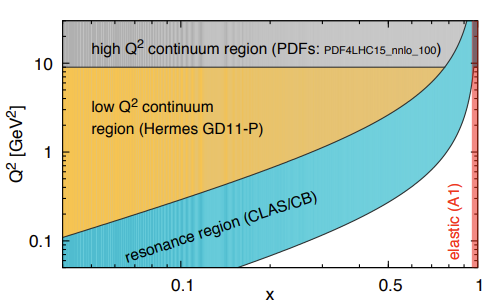
\includegraphics[width=0.89\textwidth]{figures/dataluxqed.png}
        \caption*{Input to construct $F_2$ and $F_L$}
        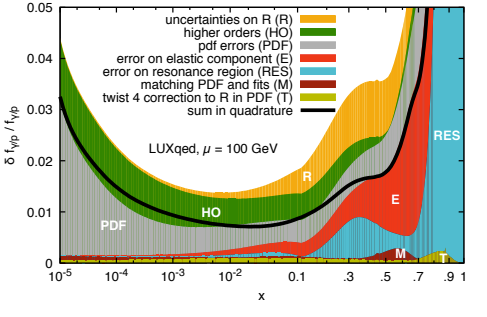
\includegraphics[width=0.89\textwidth]{figures/luxQED_uncs.png}
        \caption*{Sources of uncertainty}
      \end{figure}
    \end{column}
  \end{columns}
\end{frame}


\begin{frame}{LUXqed PDF determinations}
  LUXqed has been used in all of the most recent QED PDFs:
  \begin{itemize}
      \item LUXqed\_plus\_PDF4LHC15 {\color{gray}\small [1607.04266]}
      \item LUXqed17\_plus\_PDF4LHC15 {\color{gray}\small [1708.01256]}
      \item MMHT2015qed {\color{gray}\small [1907.02750]}
      \item NNPDF3.1luxQED {\color{gray}\small [1712.07053]}
      \item CT18lux and CT18qed {\color{gray}\small [2106.10299]}
      \item MSHT20QED {\color{gray}\small [2111.05357]}
      \item MSHT20qed\_an3lo {\color{gray}\small [2312.07665]}
      \item NNPDF4.0QED {\color{gray}\small [2401.08749 ]}
  \end{itemize}
\end{frame}

% \begin{frame}{Results: photon PDF and luminosity}
%   \begin{center}
%     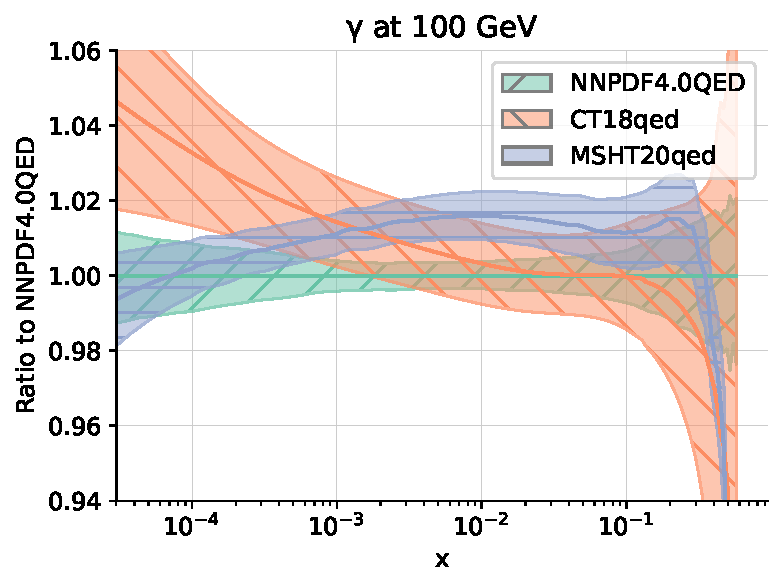
\includegraphics[width=0.3\textwidth]{figures/photon_comparison.pdf}
%     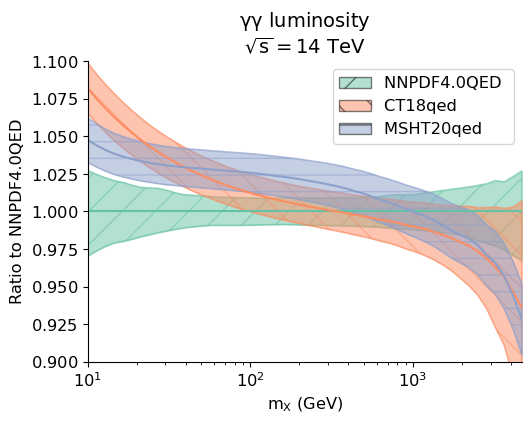
\includegraphics[width=0.3\textwidth]{figures/pp_lumi_comparison.png}
%     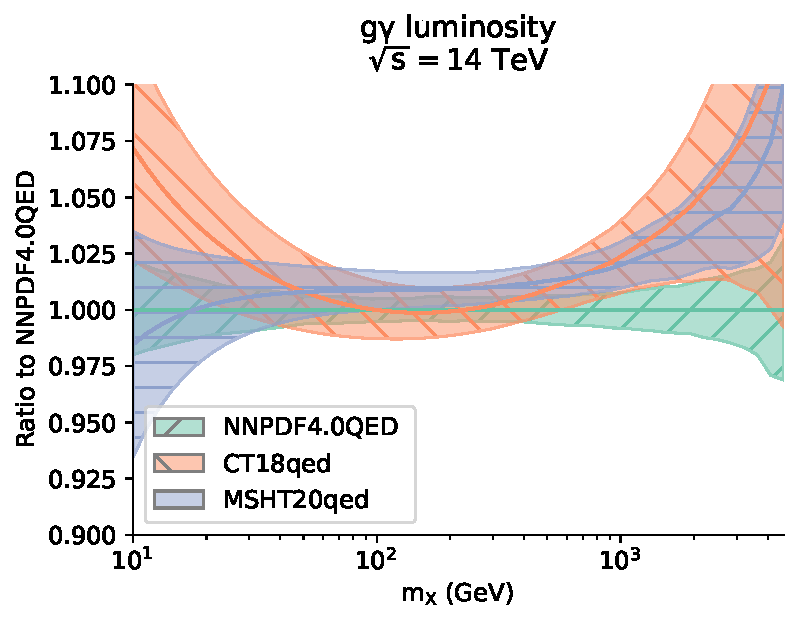
\includegraphics[width=0.3\textwidth]{figures/gp_lumi_comparison.pdf}
%   \end{center}
%   \begin{itemize}
%     \item Because all groups use the luxQED formalism, the photon PDFs agree at percent level
%     \item Luminosity generally in agreement, but differ at very small and very large invariant mass
%   \end{itemize}
% \end{frame}


% ============================================================================


\begin{frame}{Incomplete higher order uncertainties covmat}
  \begin{itemize}
    \item We construct an IHOU matrix following a similar approach by varying the subleading functions
    \item IHOU are independent of MHOU so the uncertainties are added in quadrature
    $$C = C_\mathrm{exp}+C_\mathrm{MHOU}+C_\mathrm{IHOU}$$
  \end{itemize}

  \begin{columns}
    \begin{column}{0.49\textwidth}
      \begin{figure}[!t]
        \centering
        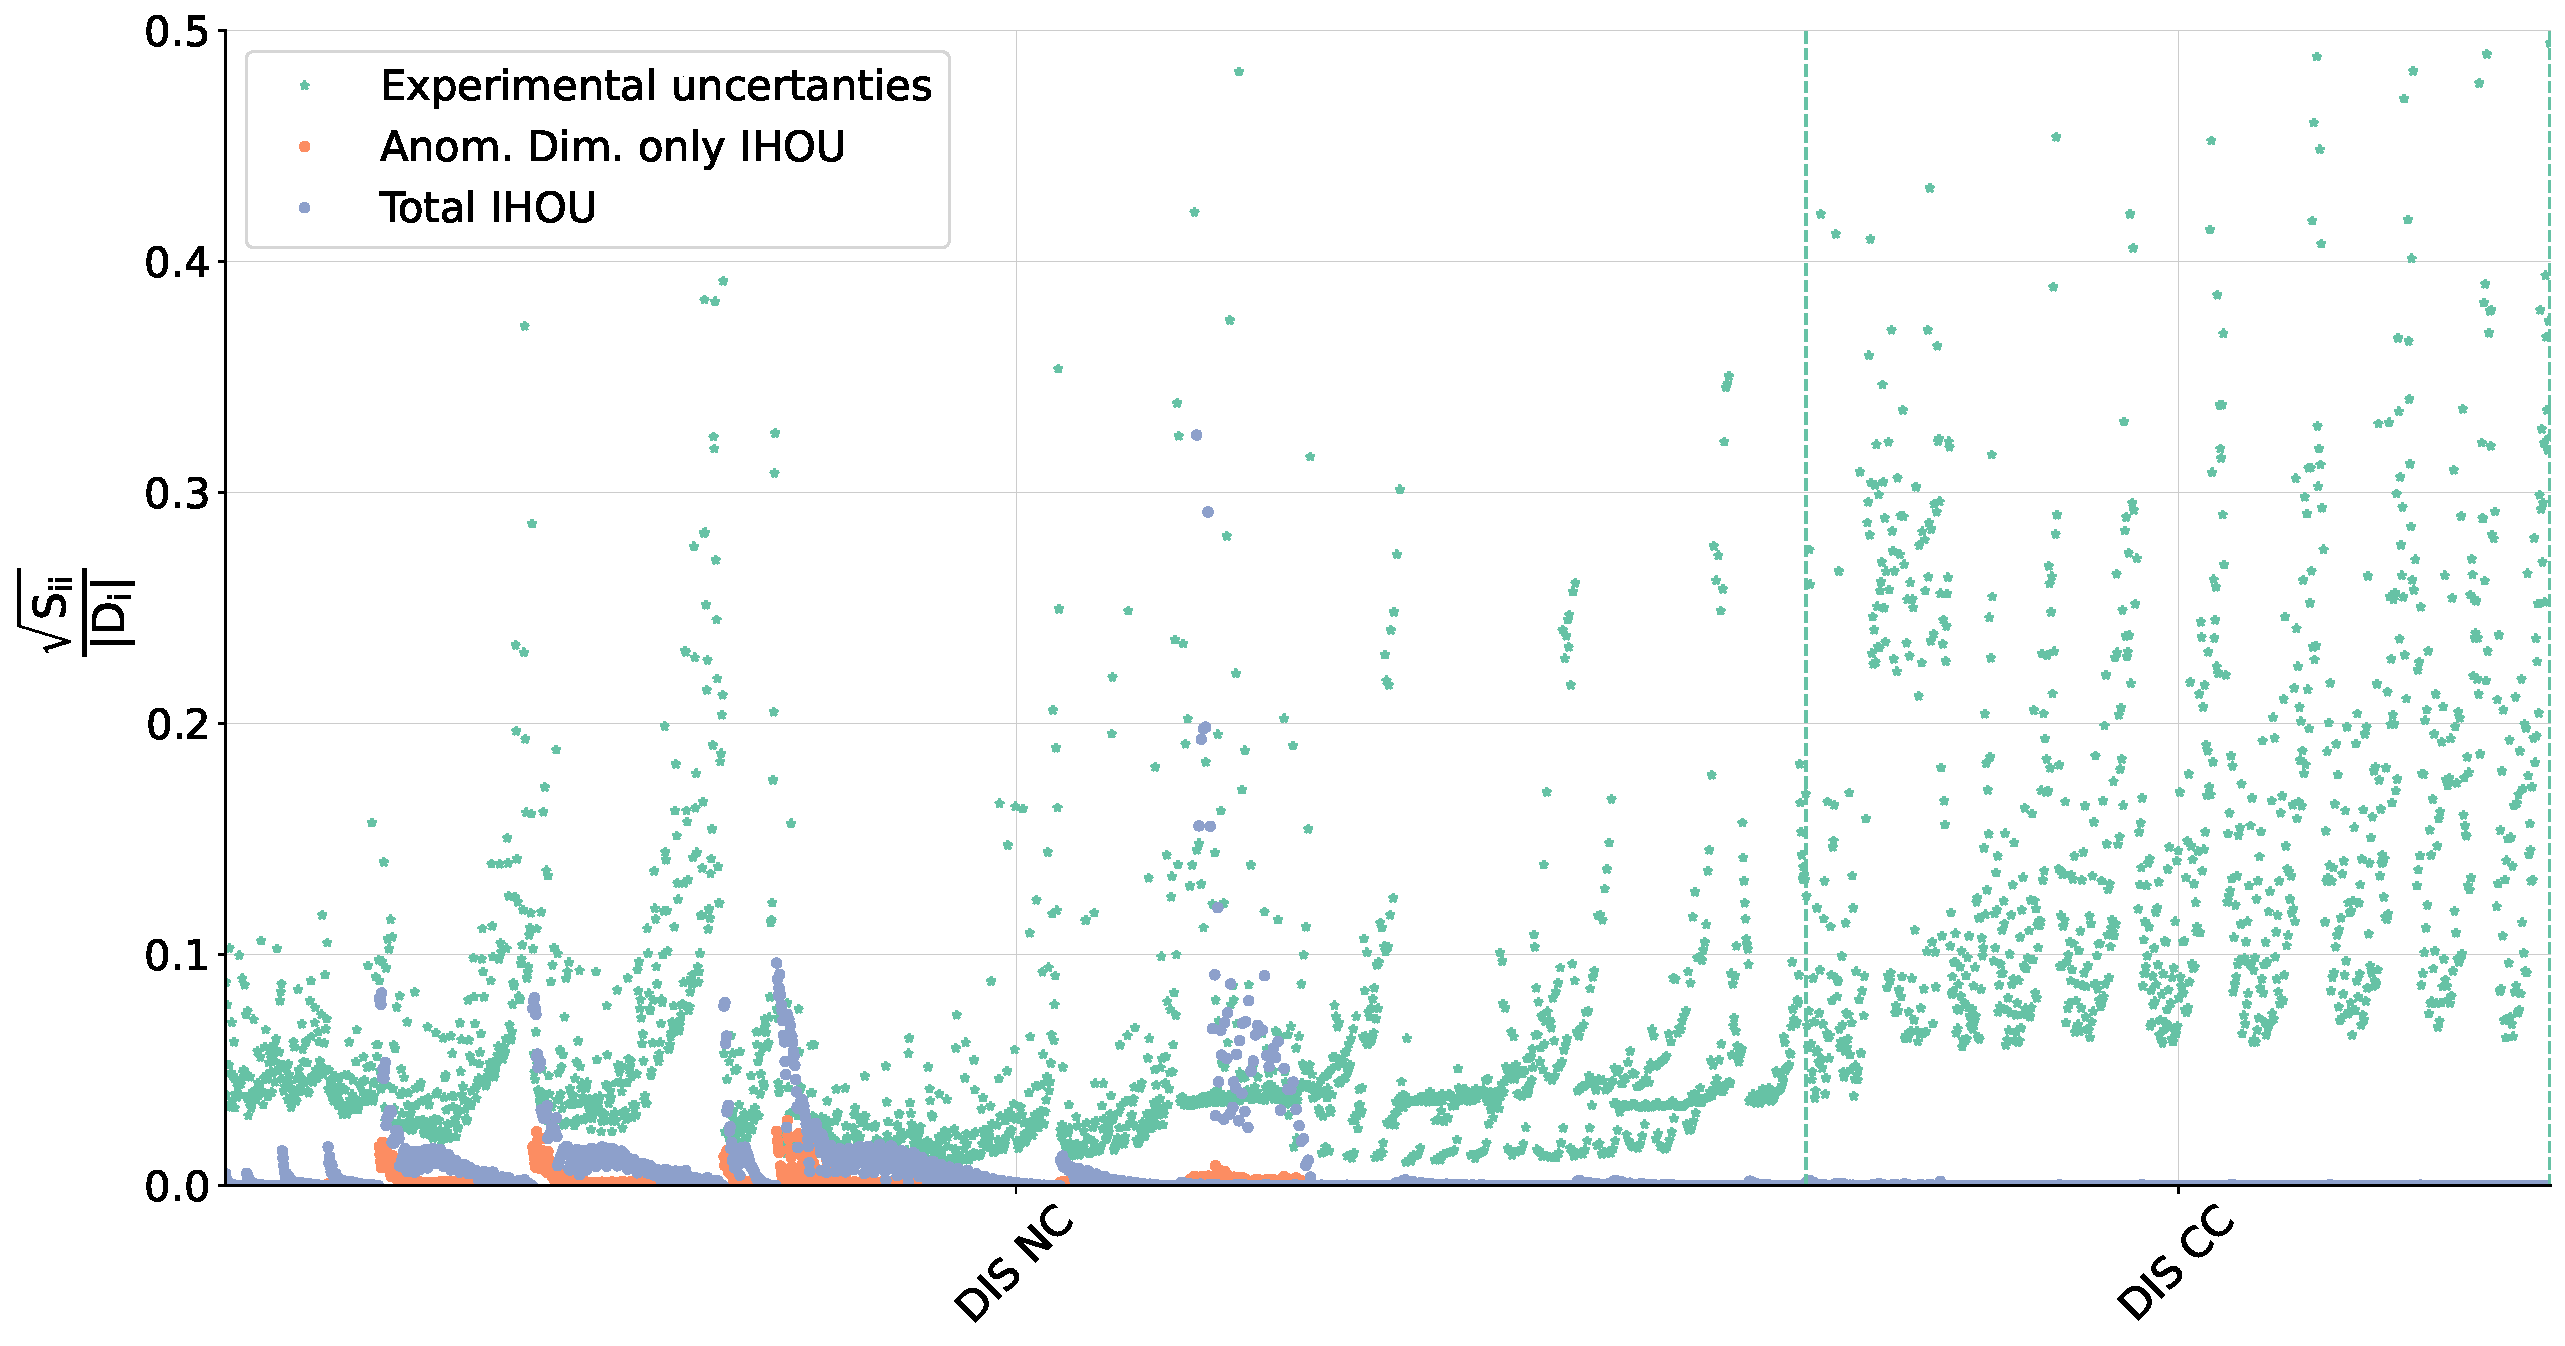
\includegraphics[width=.9\textwidth]{figures/diag_cov_dis_ihou.pdf}
        \caption*{IHOU have a large effect on small-$x$, low-$Q$ DIS data
        }
      \end{figure}
    \end{column}
    \begin{column}{0.49\textwidth}
      \begin{figure}[!t]
        \centering
        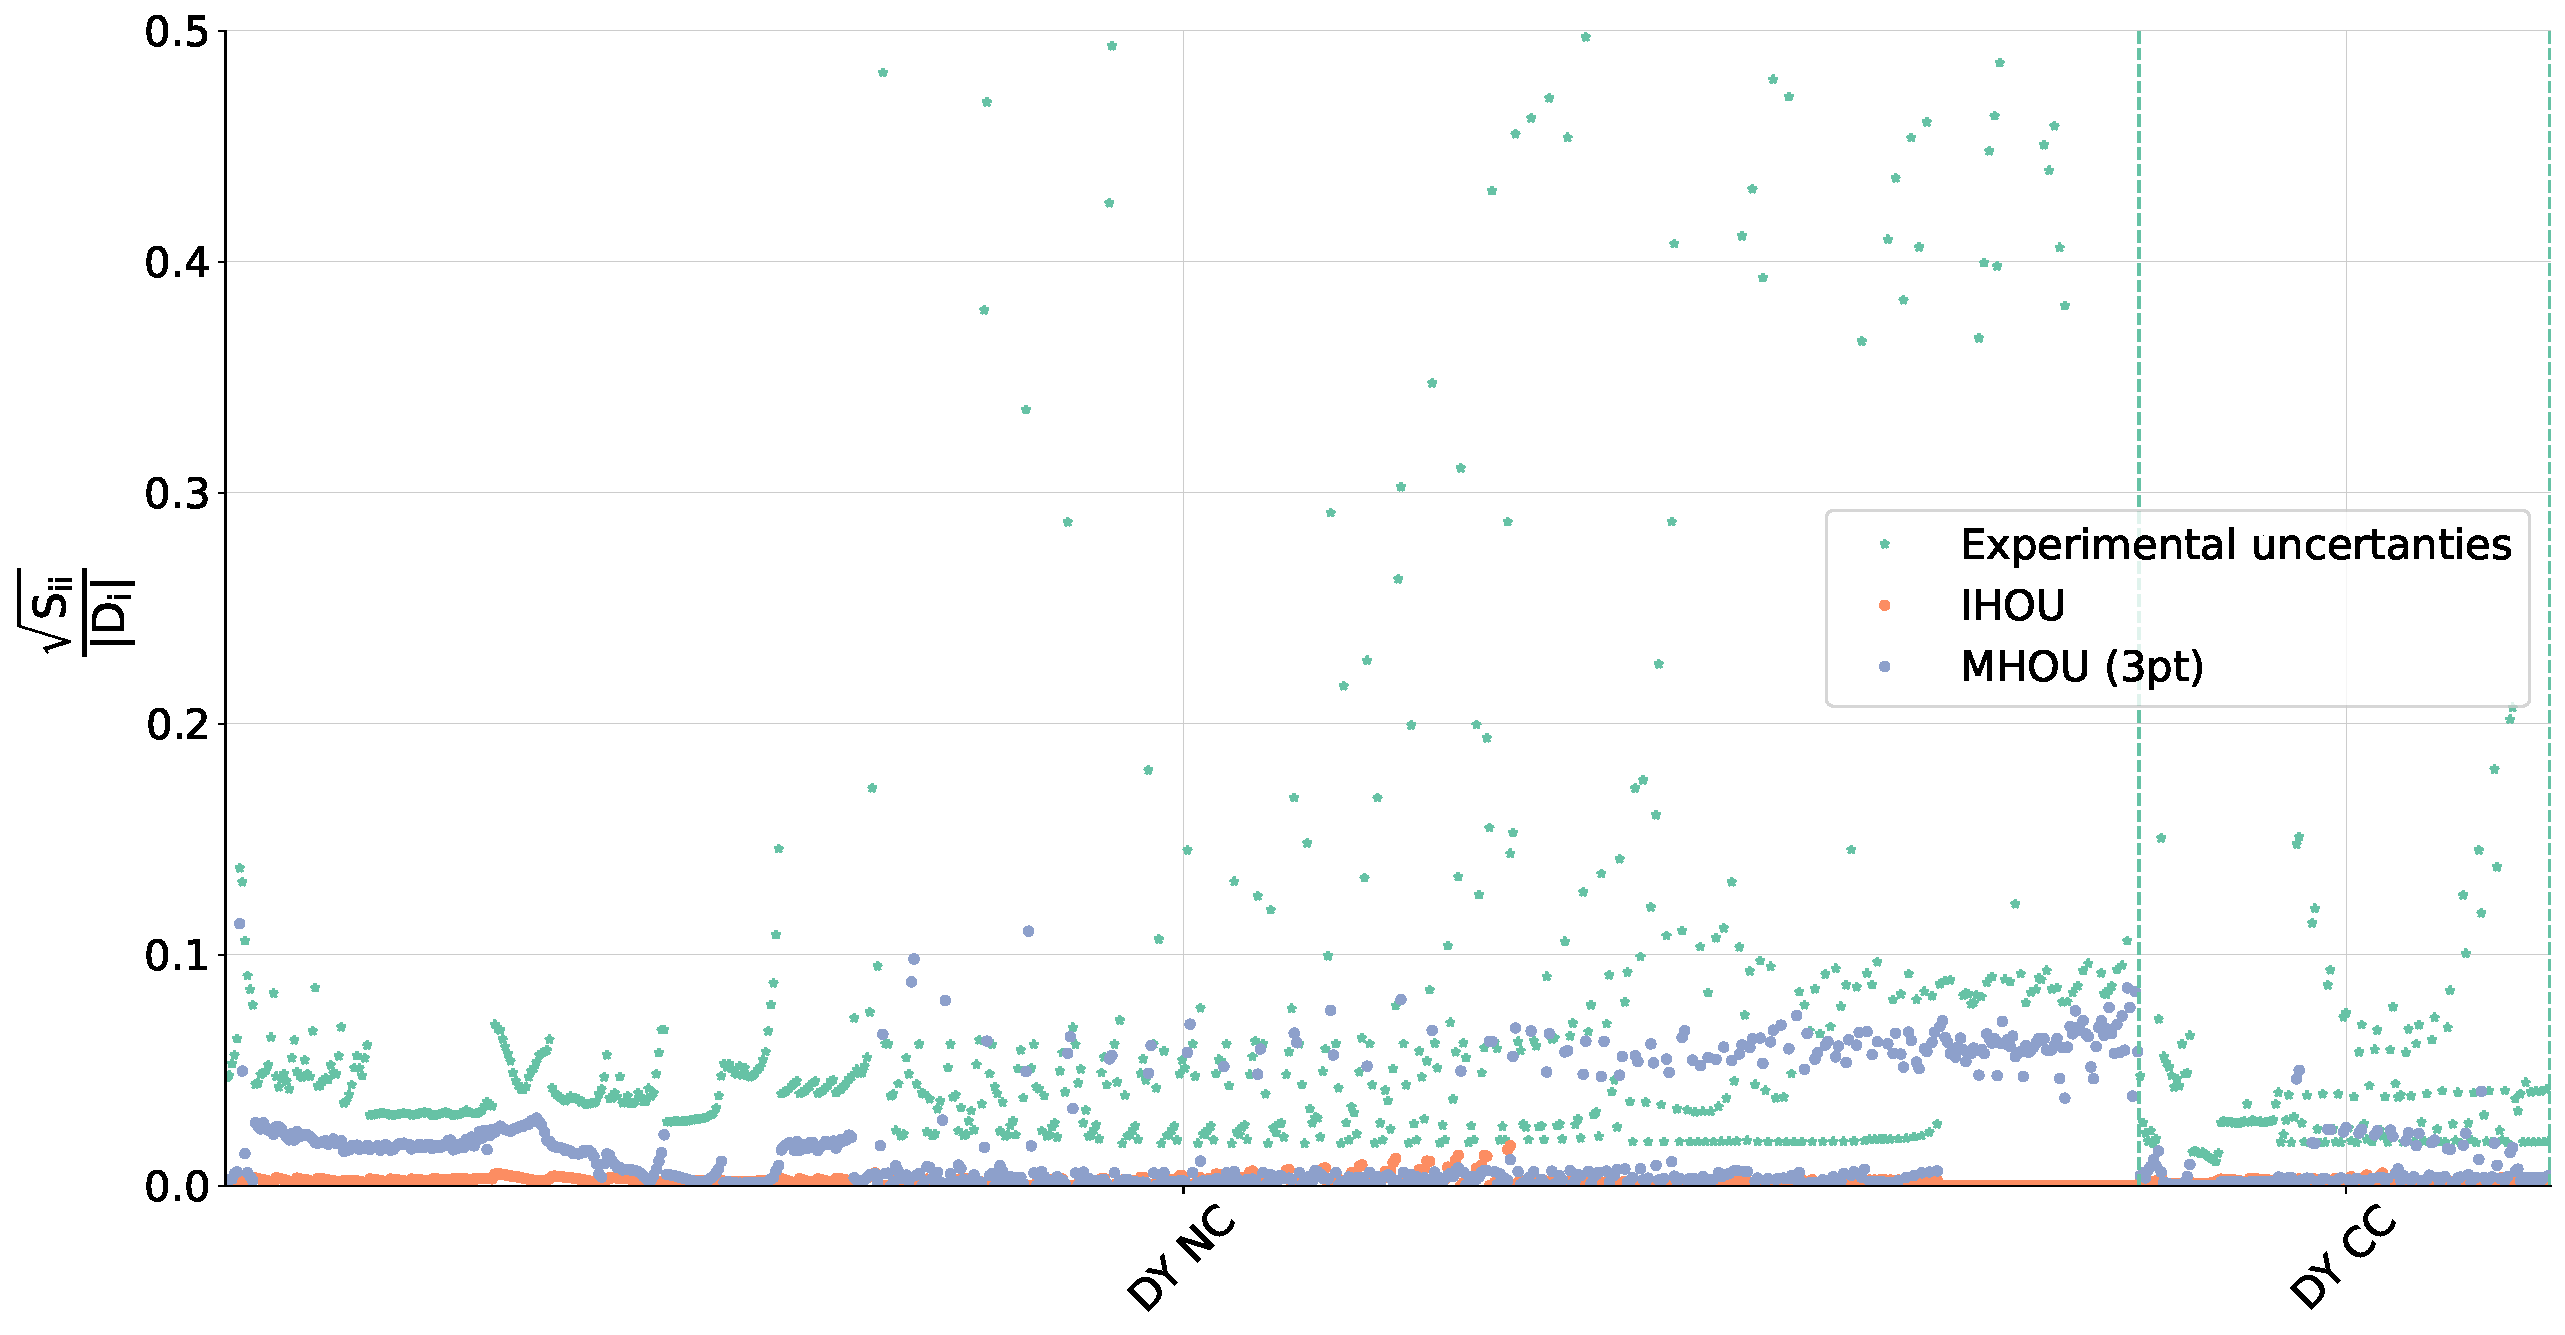
\includegraphics[width=.9\textwidth]{figures/diag_cov_dy_ihou_3pt_mhou.pdf}
        \caption*{NNLO MHOU included where N3LO not available \\
          MHOU can similar magnitude as the experimental uncertainty
        }
      \end{figure}
    \end{column}
  \end{columns}


\end{frame}

% \begin{frame}{Magnitude of theory uncertainties}
% % show that for certain processes th unc is of same size as exp unc.
% \end{frame}

% ============================================================================

\begin{frame}{Impact of MHOUs at N3LO}
  \begin{figure}[!t]
    \centering
    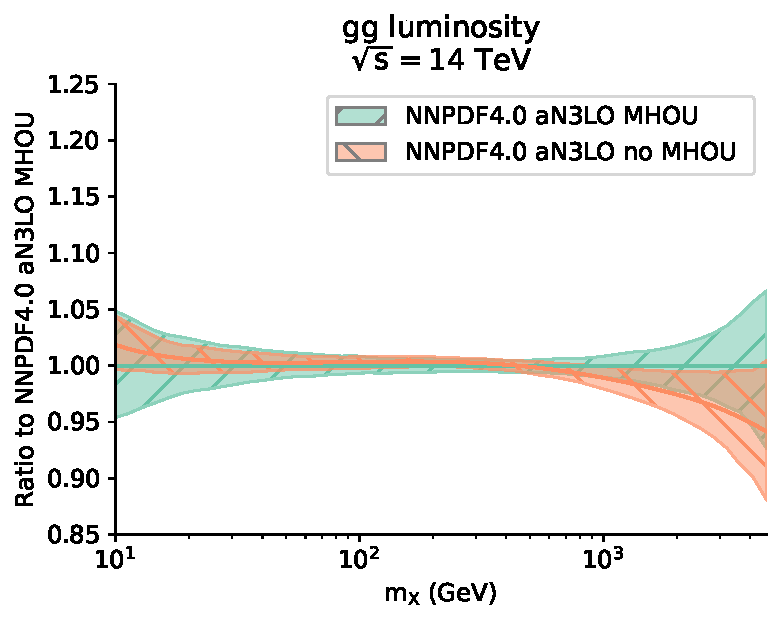
\includegraphics[width=0.45\textwidth]{figures/gg_plot_lumi1d.pdf}
    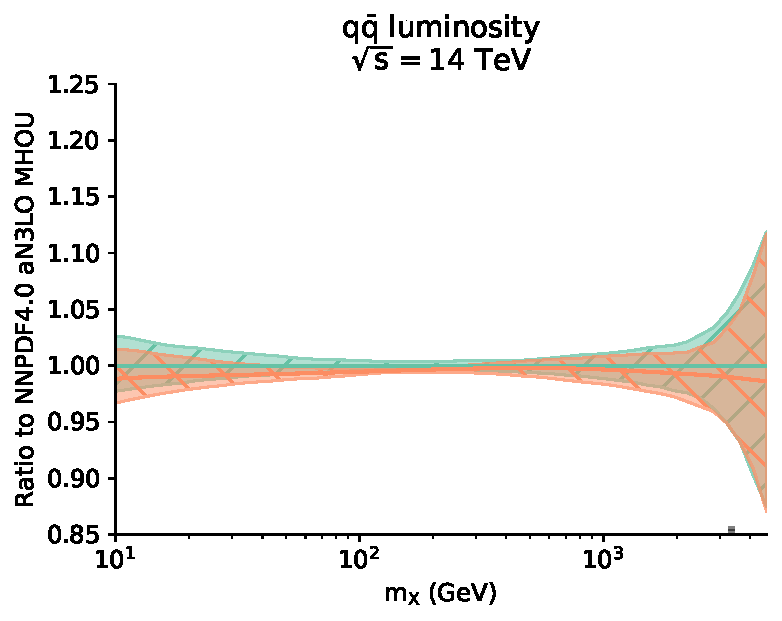
\includegraphics[width=0.45\textwidth]{figures/qqbar_plot_lumi1d.pdf}
  \end{figure}
  \begin{itemize}
    \item Non-negligible impact of MHOUs even at N3LO
    \item[$\Rightarrow$] reason to include exact N3LO calculations for hadronic processes
  \end{itemize}
\end{frame}


% \begin{frame}{Comparison to MSHT20}
%   \begin{figure}[!t]
%     \centering
%     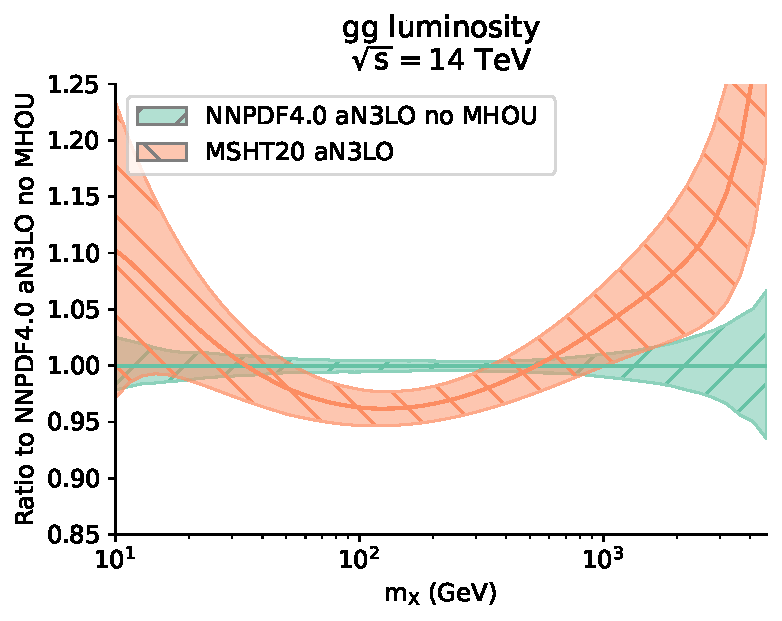
\includegraphics[width=0.45\textwidth]{figures/gg_plot_lumi1d_msht20.pdf}
%     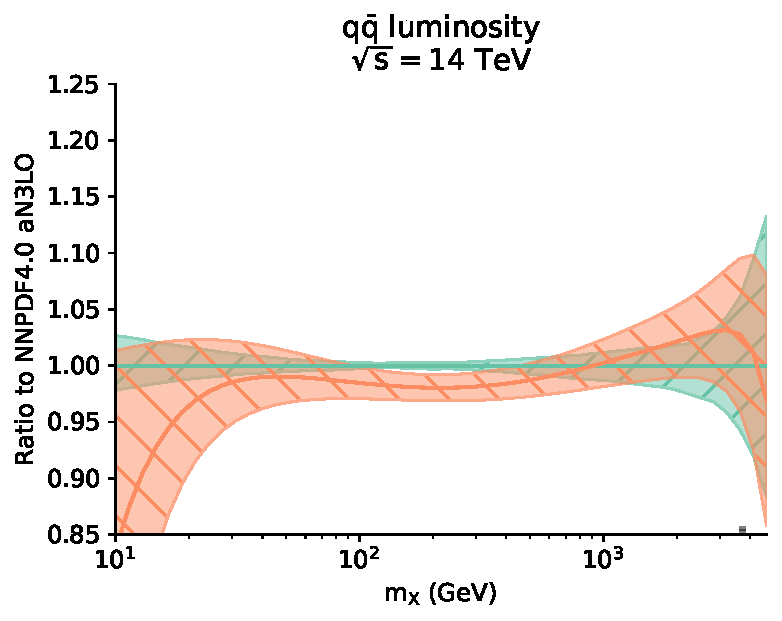
\includegraphics[width=0.45\textwidth]{figures/qqbar_plot_lumi1d_msht20.pdf}
%   \end{figure}
%   \begin{itemize}
%     \item Good agreement with MSHT20 for the quark luminosities
%     \item Also for gluon luminosities, except around the Higgs mass and high-mass
%     \item Similar data but different methodology (including splitting function parametrization)
%   \end{itemize}
% \end{frame}



\end{document}
